\documentclass[tikz, border=10pt]{standalone}
\tikzset{
    vertex/.style = {
        circle,
        fill            = black,
        outer sep = 15pt,
        inner sep = 15pt,
    }
}
\begin{document}
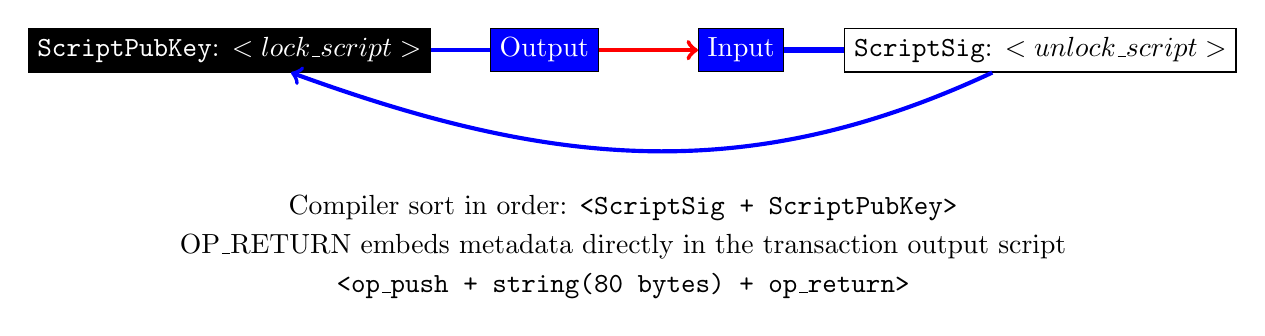
\begin{tikzpicture}
  % Coinbase

  \node[draw,fill=black,text=white] (scpk0) at (0,0) {\texttt{ScriptPubKey}: $<lock\_script>$};

  \node[draw,fill=blue,text=white] (out0) at (4,0) {Output};

  \draw[-,draw=blue,line width=1.5pt] (scpk0) to (out0);
  

  \node[draw,fill=blue,text=white] (in0) at (6.5,0) {Input};

  \draw[->,draw=red,ultra thick] (out0) to (in0);

  \node[draw] (scsg1) at (10.3,0) {\texttt{ScriptSig}: $<unlock\_script>$};

  \draw[<-,draw=blue,line width=1.5pt] (scpk0) to[in= 205,out=-20] (scsg1);

  \draw[-,draw=blue,line width=2pt] (in0) to (scsg1);

 
%   \node () at (8.8,0) {...};
  
  \node at (5, -2) {Compiler sort in order: \texttt{<ScriptSig + ScriptPubKey>}};
  \node at (5, -2.5) {OP\_RETURN embeds metadata directly in the transaction output script};
  \node at (5, -3) {\texttt{<op\_push + string(80 bytes) + op\_return>}};
  
    

\end{tikzpicture}
\end{document}